\documentclass[aspectratio=169,12pt]{beamer}
\usetheme{Madrid}
\usecolortheme{dolphin}
\usefonttheme{professionalfonts}
\setbeamertemplate{navigation symbols}{}
\setbeamertemplate{footline}{}

\usepackage[T1]{fontenc}
\usepackage[utf8]{inputenc}
\usepackage{graphicx}
\usepackage{amsmath,amssymb}
\usepackage{hyperref}
\usepackage{physics}

\title[Bell Inequalities]{Bell Inequalities}
\author{JAMOTTE Maxime, SCHOONEN Cédric}
\institute{Digital Learning Hub}
\date{}

\begin{document}

\begin{frame}
  \titlepage
\end{frame}

\begin{frame}{Table of Contents}
  \tableofcontents
\end{frame}

\section{EPR Paradox}

\begin{frame}{EPR Paradox: Setup}
  \begin{columns}[T]
    \begin{column}{0.55\textwidth}
      Entangled state produced by a source and shared between Alice and Bob:
      \[
        \ket{\psi_{AB}} = \frac{\ket{00} + \ket{11}}{\sqrt{2}} \sim \frac{\ket{++} + \ket{--}}{\sqrt{2}}
      \]
    \end{column}
    \begin{column}{0.4\textwidth}
      \centering
      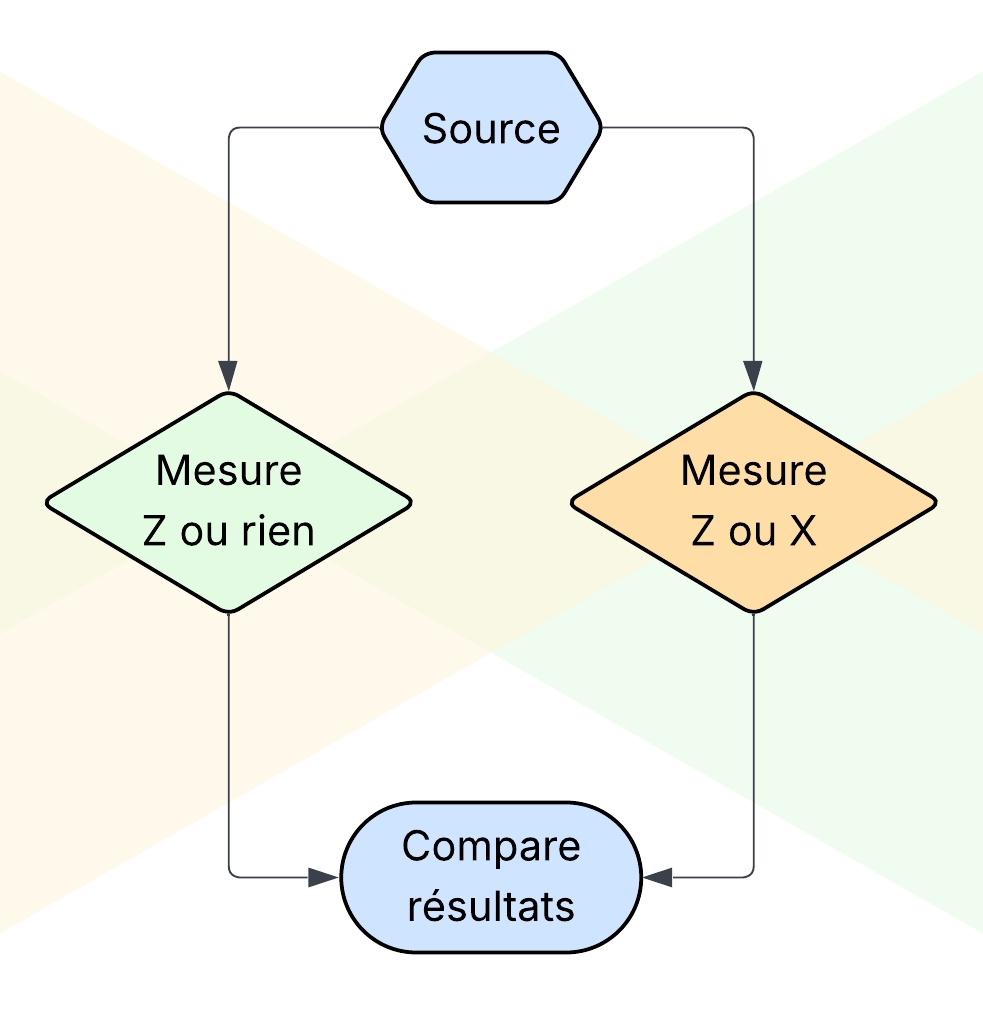
\includegraphics[width=\linewidth]{../figures/epr.png}
    \end{column}
  \end{columns}
\end{frame}

\begin{frame}{Bob's measurements alone}
  If Bob alone performs measurements, he always has a $50\%$ chance of obtaining one of the two possible states ($\ket 0$ or $\ket 1$ in the $Z$ basis, and $\ket +$ or $\ket -$ in the $X$ basis).
  
  \bigskip
  The measured averages are therefore zero:
  \[
    \langle Z_B \rangle = \left( \frac{\bra{00} + \bra{11}}{\sqrt{2}} \right) \left( \frac{\ket{00} + (-1) \ket{11}}{\sqrt{2}} \right) = 0
  \]
  \[
    \langle X_B \rangle = \left( \frac{\bra{00} + \bra{11}}{\sqrt{2}} \right) \left( \frac{\ket{01} + \ket{10}}{\sqrt{2}} \right) = 0
  \]
\end{frame}

\begin{frame}{Correlations with Alice}
  However, if Alice performs measurements in the $Z$ basis, Bob will find (once Alice has shared her results with him) that his results are totally correlated with Alice's.
  
  \bigskip
  His measurements performed in the $Z$ basis are identical to Alice's, as if Alice's measurements had influenced his (or vice versa).
  \[
    \langle Z_AZ_B \rangle = \left( \frac{\bra{00} + \bra{11}}{\sqrt{2}} \right) \left( \frac{\ket{00} + (-1)^2 \ket{11}}{\sqrt{2}} \right) = 1
  \]
  \[
    \langle Z_AX_B \rangle = \left( \frac{\bra{00} + \bra{11}}{\sqrt{2}} \right) \left( \frac{\ket{01} +(-1) \ket{10}}{\sqrt{2}} \right) = 0
  \]
\end{frame}

\begin{frame}{EPR Paradox}
  \textbf{Question:} How can Bob's results be correlated with Alice's, when Bob has no information about the measurements performed by Alice?
  
  \bigskip
  This seems to contradict the principle of \textit{locality} (no influence can propagate faster than light).

  \bigskip
  \textbf{EPR hypothesis (1935):} Quantum mechanics is incomplete. There would exist local hidden variables that predetermine the measurement results.
\end{frame}

\section{Hidden variables}

\begin{frame}{Hidden variables}
  \textbf{Defended idea:} The probabilities $|\langle 0 | \psi \rangle|^2$ and $|\langle 1 | \psi \rangle|^2$ reflect an uncertainty about the nature of the state $\ket\psi$.
  
  \bigskip
  There would be no superposition of states, but simply states whose exact nature we do not know (revealed upon measurement).
  
  \bigskip
  A more fundamental theory than quantum mechanics would describe exactly the measurement result of an observable.
\end{frame}

\begin{frame}{Example of a hidden variable}
  Let us take for example the following superposition:
  \[
    \ket\psi = \frac{\ket 0 + \ket 1}{\sqrt{2}}
  \]
  
  The probability of measuring the value $+1$ for the observable $Z$ is:
  \[
    p(+1) = |\langle 0 | \psi \rangle|^2 = \frac 12
  \]
  
  The hidden variable hypothesis assumes that the measurement result of $Z$, $z = \pm 1$, would be pre-determined and encoded in the quantum state.
\end{frame}

\begin{frame}{Hidden variable (continued)}
  The quantum state, $\ket{\psi^{(z)}}$, would in reality be either $\ket{\psi^{(+1)}} = \ket 0$ or $\ket{\psi^{(-1)}} = \ket 1$.
  
  \bigskip
  The probability $1/2$ of measuring $z=+1$ simply reflects the probability that this hidden variable equals $+1$:
  \[
    p(+1) = |\langle 0 | \psi^{(z)} \rangle|^2 = 
    \begin{cases}
        1 \quad \text{ si } z=+1 \\
        0 \quad \text{ si } z=-1
    \end{cases}
    \quad
    = p(z=+1)
  \]
\end{frame}

\begin{frame}{Hidden variables and entanglement}
  The correlations observed for entangled states,
  \[
    \ket{\psi_{AB}} = \frac{\ket{00} + \ket{11}}{\sqrt{2}}
  \]
  \[
    \langle Z_AZ_B \rangle = \left( \frac{\bra{00} + \bra{11}}{\sqrt{2}} \right) \left( \frac{\ket{00} + (-1)^2 \ket{11}}{\sqrt{2}} \right) = 1
  \]
  
  would also be explained by the pre-encoded values of the hidden variable:
  \[
    \ket{\psi_{AB}} = 
    \begin{cases}
        \ket{\psi_A^{(+1)}}\otimes\ket{\psi_B^{(+1)}} \quad \text{ si } z=+1 \\
        \ket{\psi_A^{(-1)}}\otimes\ket{\psi_B^{(-1)}} \quad \text{ si } z=-1
    \end{cases}
  \]
\end{frame}

\section{Statistical test (CHSH)}

\begin{frame}{Statistical test (CHSH)}
  \begin{columns}[T]
    \begin{column}{0.55\textwidth}
      The source emits states $\ket{\psi_A}$ and $\ket{\psi_B}$ towards Alice and Bob, respectively.
      
      \bigskip
      Alice decides to measure an observable chosen from $A_0, A_1$, and Bob does the same on his side with $B_0,B_1$.
      
      \bigskip
      Alice and Bob are far enough apart that the result of one does not influence the measurement of the other.
    \end{column}
    \begin{column}{0.4\textwidth}
      \centering
      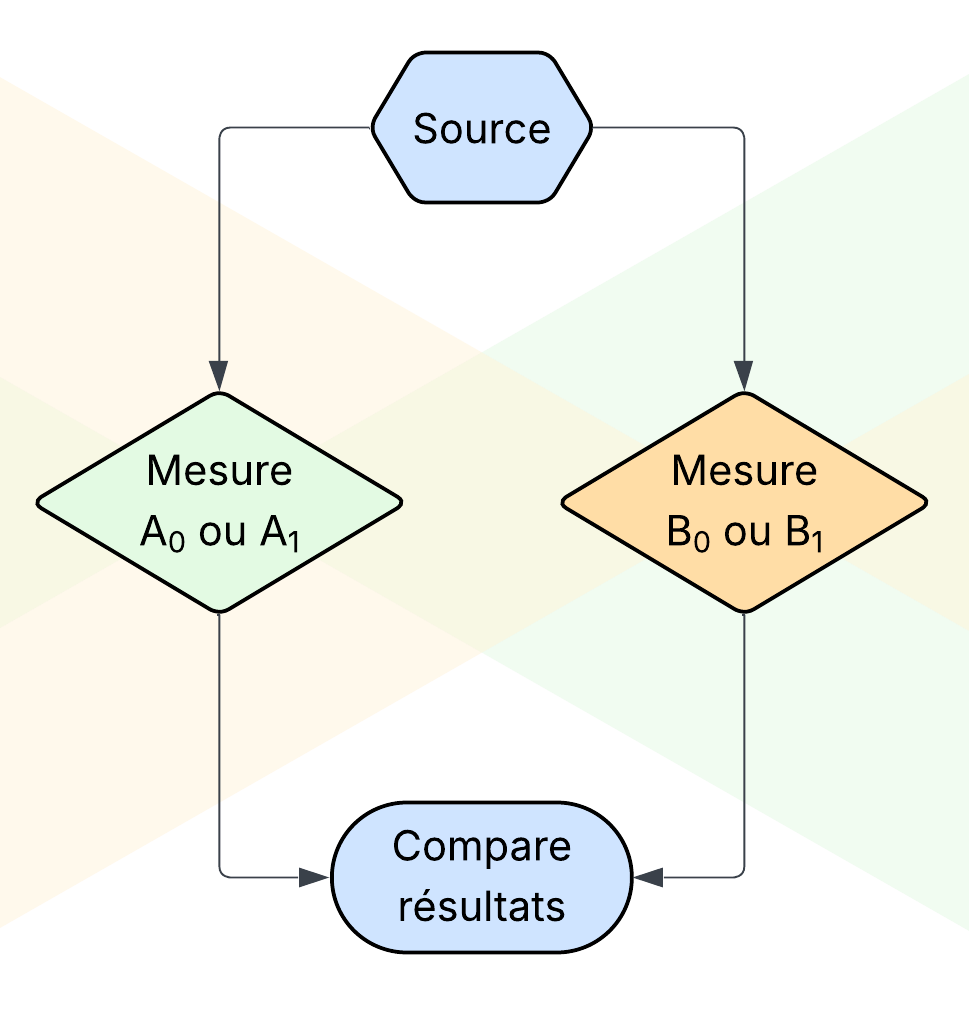
\includegraphics[width=\linewidth]{../figures/chsh.png}
    \end{column}
  \end{columns}
\end{frame}

\begin{frame}{Correlation analysis}
  The measurement results as well as the chosen observables are collected and analyzed a posteriori.
  
  \bigskip
  We then compute the correlations $\langle A_iB_j \rangle$ and evaluate
  \[
    S = \langle A_0B_0 \rangle + \langle A_0B_1 \rangle + \langle A_1B_0 \rangle - \langle A_1B_1 \rangle
  \]
\end{frame}

\begin{frame}{CHSH Inequality}
  If there exist hidden variables $a_0,a_1,b_0,b_1$ predetermining the measurement results of $A_0,A_1,B_0,B_1$, then the average combination $S$ will evaluate to
  \begin{align*}
    S &= \sum_{a_0,a_1,b_0,b_1} p(a_0,a_1,b_0,b_1) \, \underbrace{(a_0b_0+ a_0b_1 + a_1b_0 - a_1b_1)}_{a_0(b_0+b_1) \, + \, a_1(b_0-b_1)}
  \end{align*}
  
  Since $b_0,b_1 = \pm 1$ we necessarily have one of the two factors $(b_0+b_1)$ or $(b_0-b_1)$ that vanishes, the other taking the value $\pm 2$.
\end{frame}

\begin{frame}{CHSH Inequality (continued)}
  Thus,
  \[
    a_0(b_0+b_1) + a_1(b_0-b_1) = \pm 2
  \]
  
  et donc
  \[
    |S| \le 2
  \]
  
  \bigskip
  This equation is called \textbf{the CHSH inequality} and is an example of a Bell inequality. It serves to test the hypothesis of the presence of hidden variables.
\end{frame}

\section{Quantum violation}

\begin{frame}{Quantum mechanics does not respect Bell inequalities}
  In the CHSH case, let us consider the following observables for Alice:
  \[
    A_0 = Z
    \qquad
    A_1 = X
  \]
  
  And these for Bob:
  \[
    B_0 = \frac{Z+X}{2}
    \qquad
    B_1 = \frac{Z-X}{2}
  \]
\end{frame}

\begin{frame}{Quantum violation (continued)}
  If the source produces the states
  \[
    \ket{\psi_{AB}} = \frac{\ket{01} - \ket{10}}{\sqrt{2}}
  \]
  
  then the correlations will be
  \[
    \langle A_0B_0 \rangle = +\frac{1}{\sqrt{2}} \qquad
    \langle A_0B_1 \rangle = +\frac{1}{\sqrt{2}}
  \]
  \[
    \langle A_1B_0 \rangle = +\frac{1}{\sqrt{2}} \qquad
    \langle A_1B_1 \rangle = -\frac{1}{\sqrt{2}}
  \]
  
  And the combination $S = 2\sqrt{2} > 2$
\end{frame}

\section{Alain Aspect's experiments}

\begin{frame}{Alain Aspect's experiments (1982)}
  Concrete implementation of the situation described in the EPR paradox, with polarized light:
  
  \begin{center}
    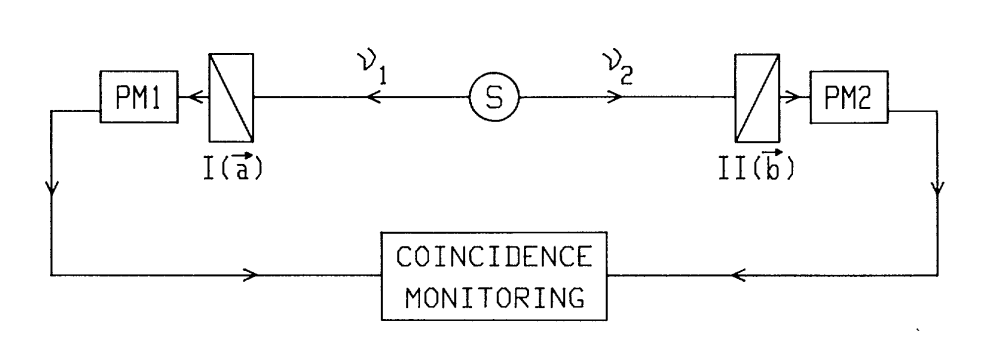
\includegraphics[width=0.7\linewidth]{../figures/aspect1.png}
  \end{center}
\end{frame}

\begin{frame}{Setting up the CHSH test}
  Setting up the CHSH statistical test:
  
  \begin{center}
    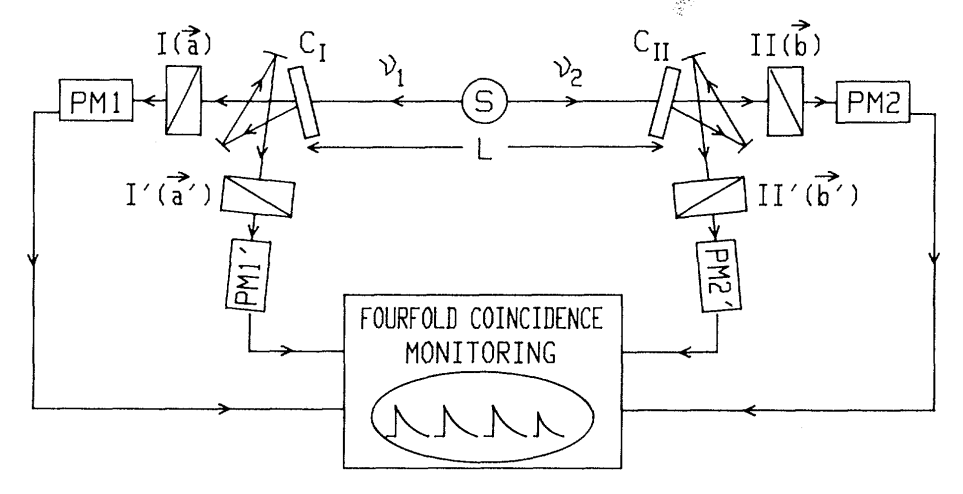
\includegraphics[width=0.7\linewidth]{../figures/aspect2.png}
  \end{center}
\end{frame}

\begin{frame}{Optical switch}
  Detail of the optical switch:
  
  \begin{center}
    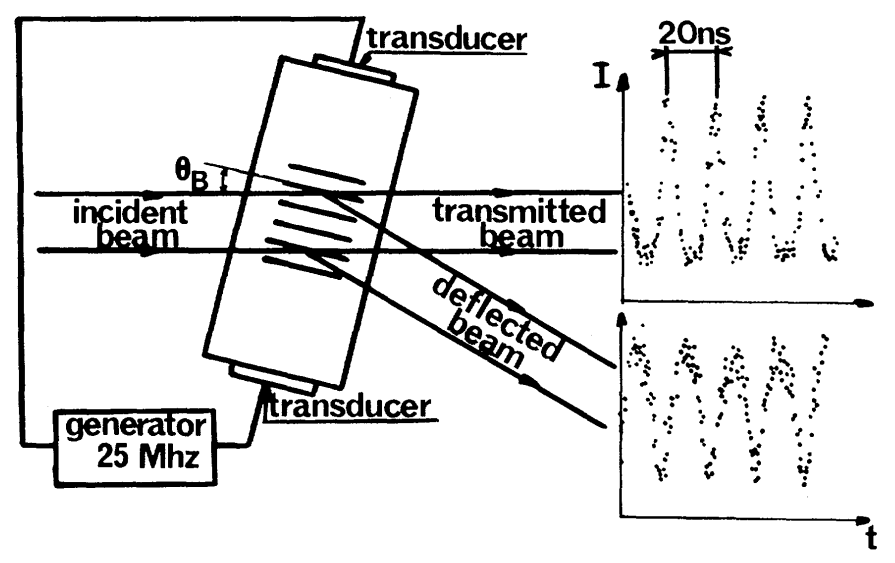
\includegraphics[width=0.7\linewidth]{../figures/aspect3.png}
  \end{center}
\end{frame}

\begin{frame}{Conclusions}
  \begin{itemize}
    \setlength{\itemsep}{0.8em}
    \item Bell inequalities allow testing the hypothesis of local hidden variables
    \item Quantum mechanics predicts a violation of these inequalities
    \item Alain Aspect's experiments (1982) confirmed the violation
    \item Nobel Prize in Physics 2022 for Aspect, Clauser and Zeilinger
  \end{itemize}
\end{frame}

\begin{frame}{Videos on the topic}
  \begin{center}
    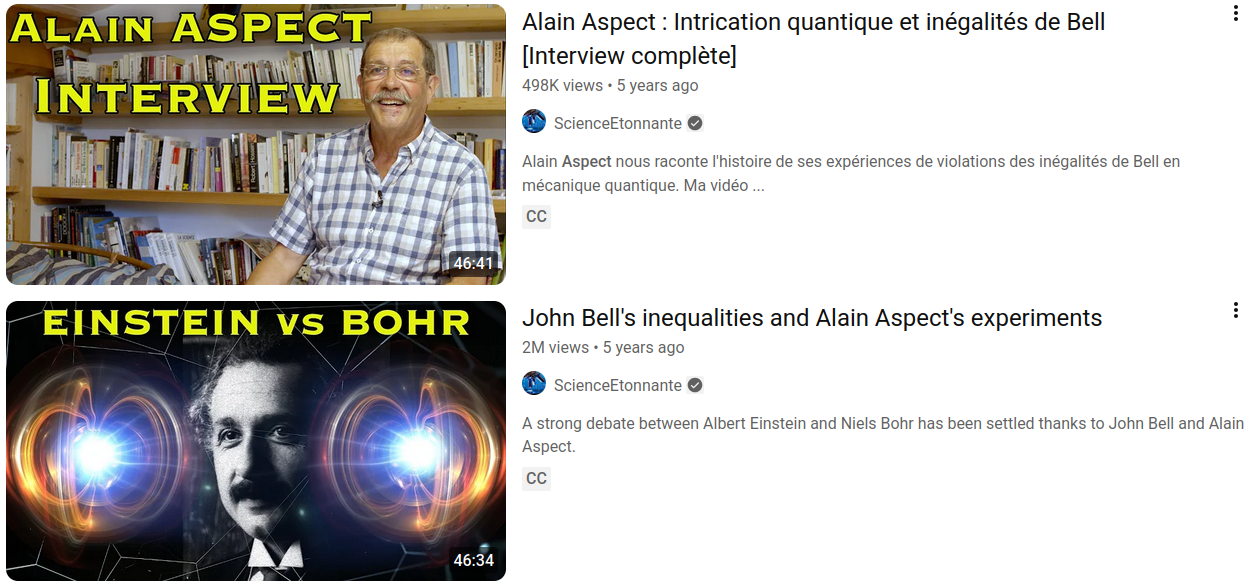
\includegraphics[width=\linewidth]{../figures/scienceetonnante.png}
  \end{center}
\end{frame}

\end{document}
